\section{\emph{Secrets}}
\label{sec:buildserver-secrets}
Dieser Abschnitt behandelt die verwendeten \emph{Secrets}. Das \emph{Secret-Objekt} oder kurz \emph{Secret} bietet eine Möglichkt zum Speichern vertraulicher Informationen wie Benutzername/Passwort, Konfigurationsdateien und viele mehr. Die Definition eines Secrets sieht wie folgt aus:

\begin{listing}[H]
	\centering
	\begin{minted}{yaml}
	apiVersion: "v1"
	kind: "Secret"
	metadata:
	  name: "test-secret"
	data: 
	  username: "dmFsdWUtMQ0K"
	  password: "dmFsdWUtMg0KDQo="
	\end{minted}
	\caption{Secret Definition}
\end{listing}

\subsection{Projekt Secrets}

In diesem Projekt werden in den diversen Builds verschiedene Secrets verwendet. Zu diesen Secrets zählen unter Anderem ein SSH-Key für GitHub und die jeweiligen Benutzernamen und Passwörter für die Kommunikation zwischen OpenShift, Jenkins und Nexus. Diese Secrets werden in OpenShift an einer zentralen Stelle verwaltet und können in Buildprozesse \emph{injeziert} werden. Durch die Injektion in z.B. Jenkins stehen diese dann in Jenkins als Umgebungsvariablen zur Verfügung.

\begin{figure}[H]
	\centering
	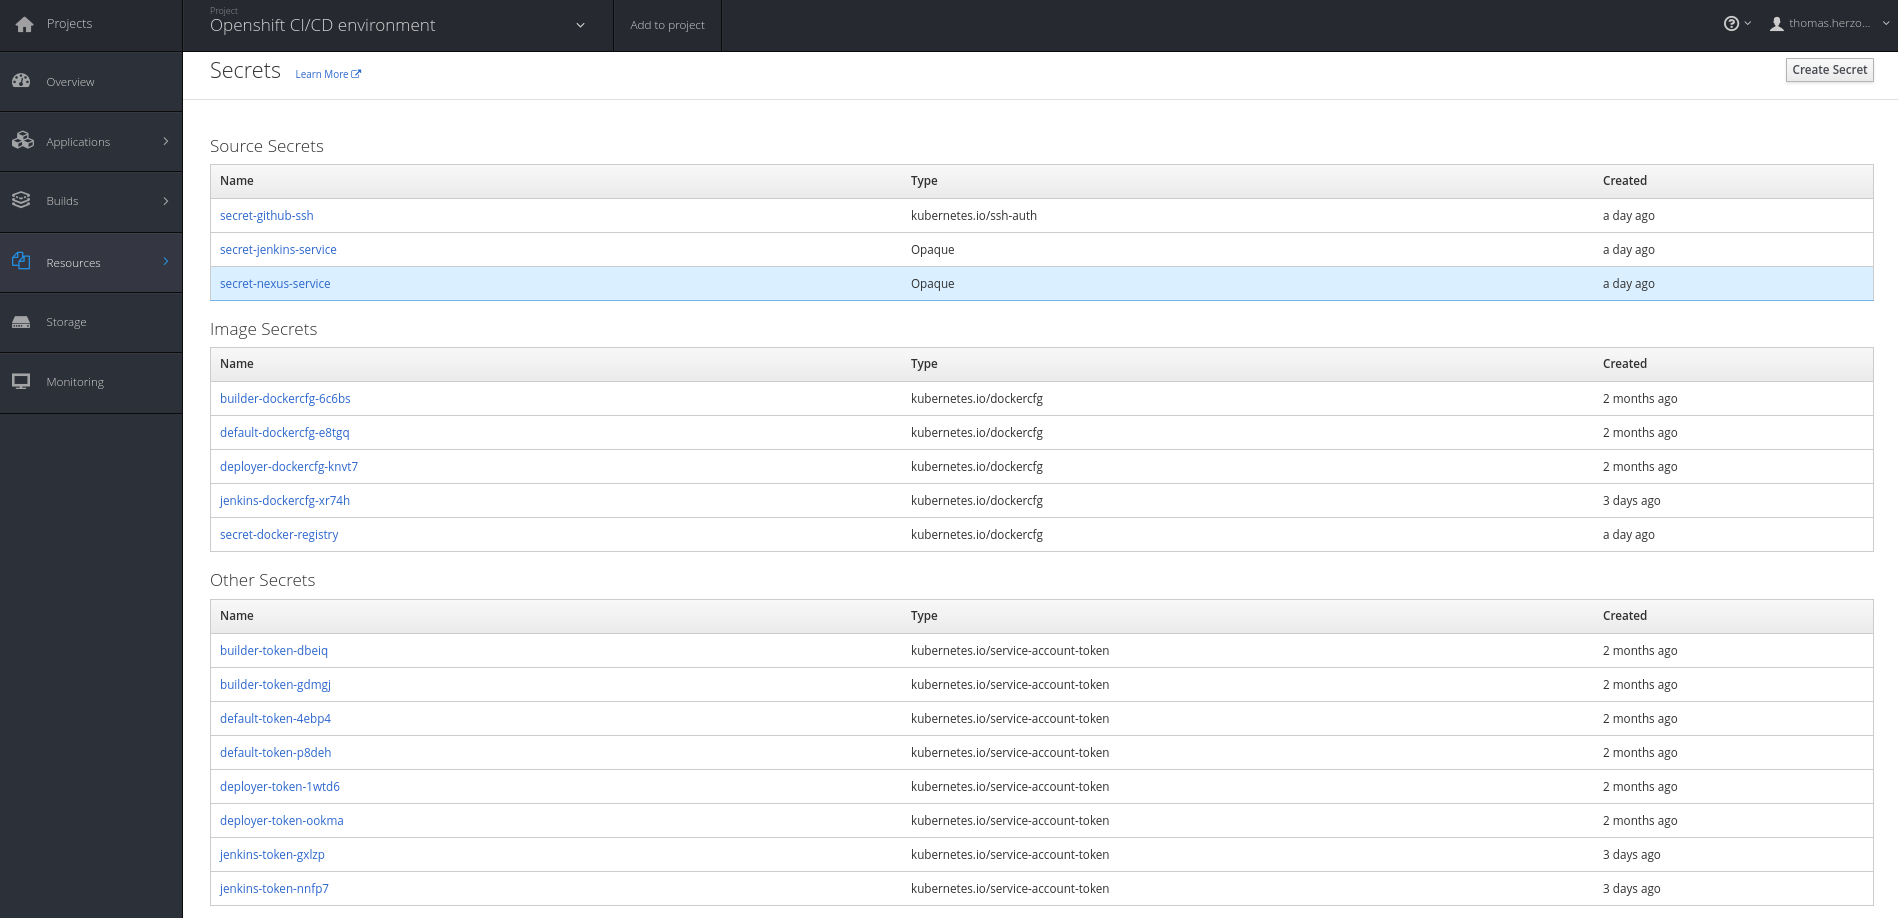
\includegraphics[scale=0.3]{image/openshift-secrets.png}
	\caption{OpenShift Secrets Übersicht}
	\label{fig:architecture}
\end{figure}